\graphicspath{{experimental_setup/fig/}}

\chapter{Experimental Setup} \label{chap:experimental_setup}
This chapter provides our research questions, and how we attempt to answer
these questions using the results of different experiments. We discuss the datasets used for
our ASR models, as well as the data used for our language model (LM).
The chapter ends with a discussion of the metric used to evaluate our ASR models.

\section{Research questions and experiments}
\subsection{Research questions}
The focus of our research is determining how to obtain the best Afrikaans and isiXhosa ASR models with limited data and computational resources.
Our approach involves fine-tuning (\ref{subsec:finetune}) the \href{https://huggingface.co/facebook/wav2vec2-xls-r-300m}{XLS-R (300M)} model using different fine-tuning strategies.
We focus on two strategies in this study. The first (\emph{basic}) strategy involves fine-tuning on one dataset (one language),
which is the typical strategy for fine-tuning XLS-R (300M). The second strategy involves fine-tuning on two datasets (two languages) seperately.
The second strategy is referred to as the \emph{sequential} fine-tuning strategy. The intent of the sequential fine-tuning strategy is
to first fine-tune on one language (e.g. Dutch), and then fine-tune on a different, but related, language (e.g. Afrikaans).
We create several models using both strategies and each model is evaluated on a validation and test set using the word error rate (WER) (\ref{subsec:wer}).
Finally, we choose the best model from both strategies for each language, add an LM (\ref{subsec:lm-boost}) to each model to boost performance, and compare their final results.

\subsection{Experiments}
For the basic fine-tuning strategy, we fine-tune using either Afrikaans or isiXhosa speech data.
For the sequential fine-tuning strategy, we fine-tune using either Dutch and then Afrikaans speech data, 
or isiZulu and then isiXhosa speech data. We chose Dutch and isiZulu, 
because Dutch is similar to Afrikaans \cite{wikipedia2023comparison_afrikaans_dutch} 
and isiZulu is similar to isiXhosa \cite{msskapstadt2023progressively_repurpose}.
We first find the best Dutch and isiZulu model by using the basic fine-tuning strategy,
and then we fine-tune those models to Afrikaans and isiXhosa respectively.

\newpage

For each experiment, we change the values of the following hyperparameters: 
\texttt{batch size}, \texttt{gradient accumulation steps}, \texttt{evaluation steps}, and \texttt{patience}.
The \texttt{evaluation steps} is the number of (gradient) steps between each evaluation on the validation set,
and the \texttt{patience} is the parameter used for early stopping \cite{wikipedia2023early_stopping}. 
We use early stopping to prevent overfitting on the training data.

\section{Data}
We use three different speech corpora\footnote{The word ``corpora'' is the plural form of the word ``corpus''.}
to create an \href{https://huggingface.co/datasets/lucas-meyer/asr_af}{Afrikaans dataset} 
and an \href{https://huggingface.co/datasets/lucas-meyer/asr_xh}{isiXhosa dataset}, which contains labeled speech recordings.
We also use one of the corpora to create Dutch and isiZulu datasets (for sequential fine-tuning).
We discuss the three corpora in the paragraphs below.

\paragraph*{NCHLT.}
The NCHLT \cite{barnard2014nchlt} corpus contains speech recordings for the eleven official South African languages.
The dataset contains approximately $200$ speakers per language.
The NCHLT recordings (on average) are the shortest of the three corpora, with most recordings being between $2$ and $6$ seconds.
Based on brief inspection, the transcription texts of this dataset contain very few words, and rarely contain full sentences.

\paragraph*{FLEURS.}
The FLEURS \cite{fleurs2022arxiv} corpus contains speech recordings for $102$ different languages, including Afrikaans, Dutch, isiXhosa, and isiZulu.
Each language has its own training, validation, and test set split.
No information is given about the number of speakers for each language.
The FLEURS recordings (on average) are the longest of the three corpora, with most recordings being between $7$ and $20$ seconds.
Based on brief inspection, the transcription texts of this dataset contain full sentences.

\paragraph*{High-quality TTS.}
The High-quality text-to-speech (TTS) \cite{hq2017} corpus contains high-quality transcribed audio data for four South African languages: Afrikaans, Sesotho, Setswana and isiXhosa.
There are nine Afrikaans speakers and 12 isiXhosa speakers.
The duration of most recordings are between $5$ and $10$ seconds.
Based on brief inspection, the transcription texts of this dataset contain mostly full sentences and a few that contain short phrases.
\\
\\
As mentioned, we select recordings from the three corpora to create the final Afrikaans and isiXhosa datasets.
Additionaly, we use the Dutch and isiZulu data from the FLEURS dataset for our sequential fine-tuning experiments.

\subsection{Approach for selecting recordings}
To optimize training and GPU memory usage, we select recordings to maintain a roughly uniform distribution in terms of their durations.
This approach mitigates the challenges of random batch selection during fine-tuning.
Since batches are selected randomly, one batch may contain much longer recordings than another batch.
Inconsistent batch durations may lead to suboptimal GPU memory allocation, leading to all of the GPU memory being used and triggering an exception.
The NCHLT dataset contains much more data than the other two datasets. However, the NCHLT recordings are much shorter and lower quality. 
Consequently, we omit a large portion of the NCHLT dataset in favor of the recordings from the other two datasets.
Figure \ref{fig:histogram1} describes the histograms of the recording durations of the two datasets without removing outliers,
Figure \ref{fig:histogram2} describes the h istograms of the recording durations of the two datasets after removing outliers.
Note that we lose a significant portion of the data. However, it allows us to use larger batch sizes during fine-tuning and as we mentioned the NCHLT
recordings are low-quality recordings of short phrases not considered to be full sentences.

\begin{figure}[!ht]
    \centering
    \begin{minipage}{.45\textwidth}
      \centering
      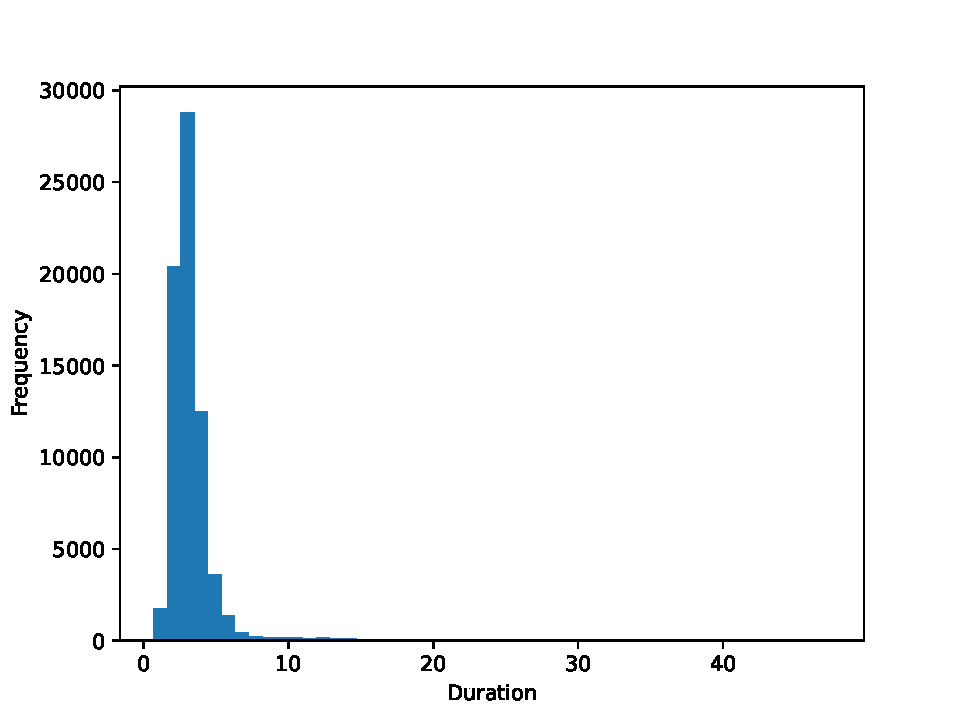
\includegraphics[width=\linewidth]{before_histogram_af.pdf}
    \end{minipage}%
    \begin{minipage}{.45\textwidth}
      \centering
      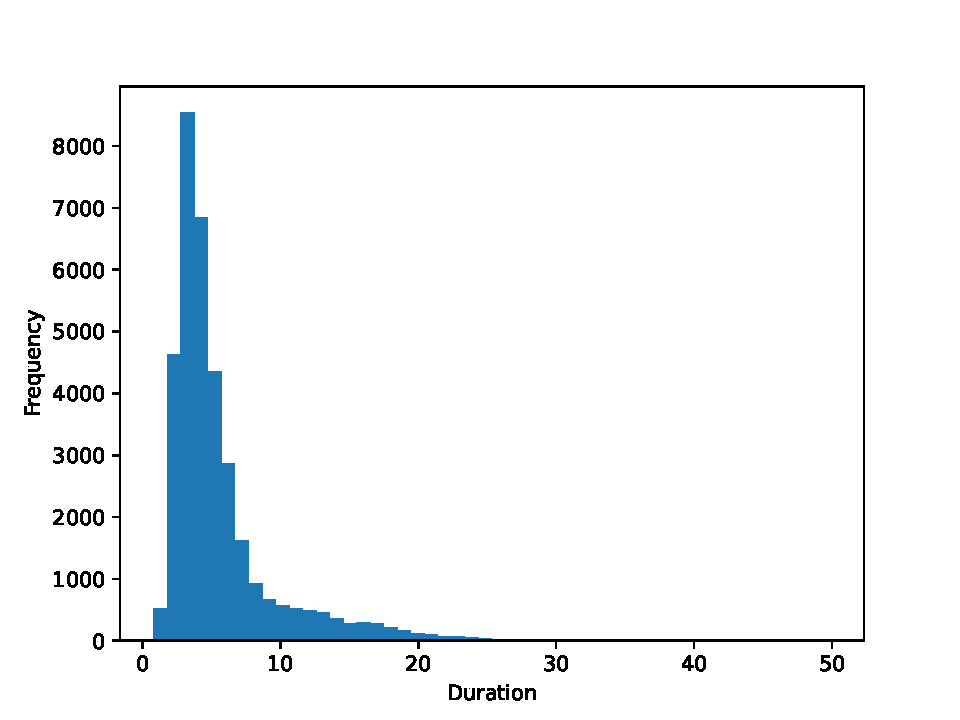
\includegraphics[width=\linewidth]{before_histogram_xh.pdf}
    \end{minipage}
    \caption{The histograms of the recording durations of the Afrikaans dataset (left) and the isiXhosa dataset (right) \textbf{without removing outliers}.}
    \label{fig:histogram1}
\end{figure}

\begin{figure}[!ht]
    \centering
    \begin{minipage}{.45\textwidth}
      \centering
      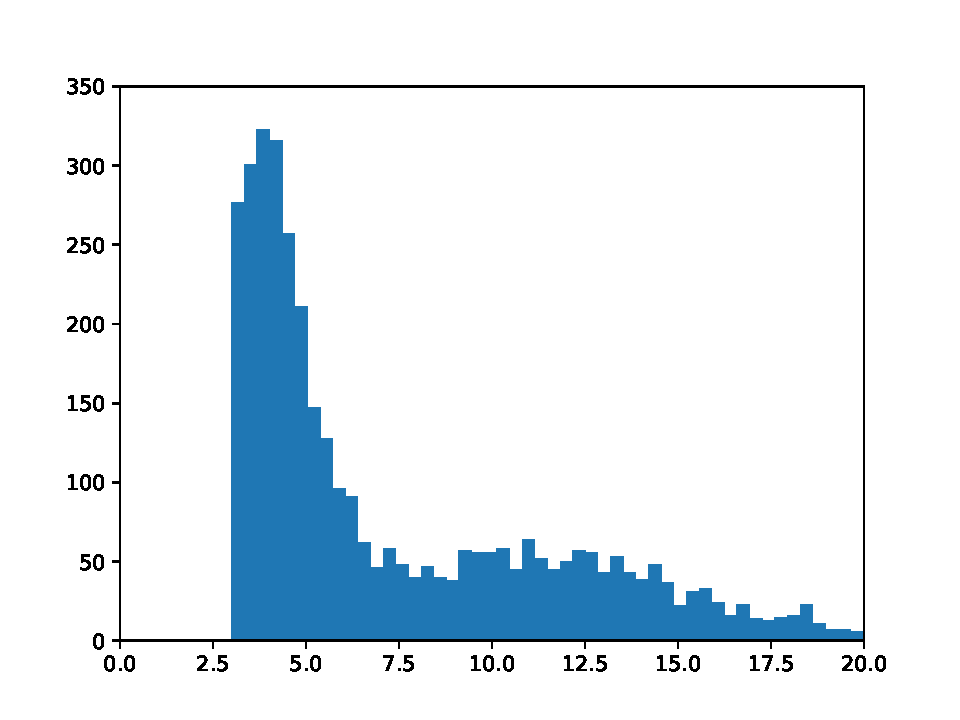
\includegraphics[width=\linewidth]{final_histogram_af.pdf}
    \end{minipage}%
    \begin{minipage}{.45\textwidth}
      \centering
      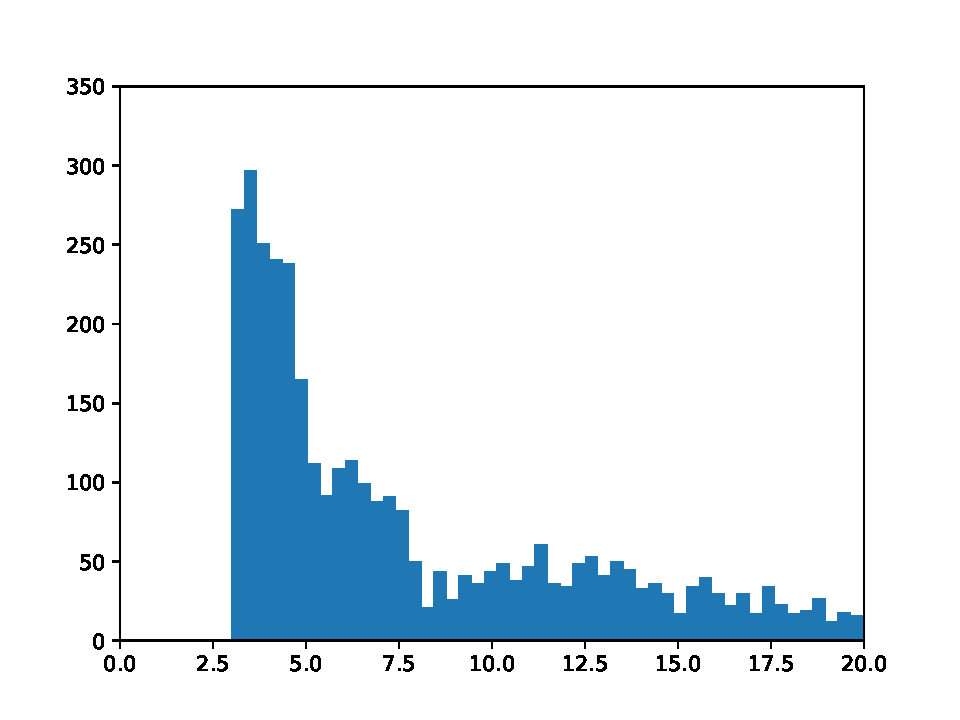
\includegraphics[width=\linewidth]{final_histogram_xh.pdf}
    \end{minipage}
    \caption{The histograms of the recording durations of the Afrikaans dataset (left) and the isiXhosa dataset (right) \textbf{after removing outliers}.}
    \label{fig:histogram2}
\end{figure}

Both datasets contain approximately $7.5$ hours of speech recordings (after removing outliers). 
Additionaly, we ensure that the validation and test sets do not contain recordings of speakers that appear in the training set (\ref{par:excl_split}).
The transcription texts are pre-processed in the same way as the LM data, which is explained in the following section.

\subsection{Language model data}
The data used for training the LM (\ref{subsec:lm-boost}) consists of \href{https://dumps.wikimedia.org/}{Wikipedia dumps}.
The text is extracted from the dumps using a tool called the WikiExtractor \cite{Wikiextractor2015}.
The text is pre-processed by converting all characters to lowercase, removing all characters that are not used in the Afrikaans
and isiXhosa language, and removing punctuation marks and other special characters.

\section{Evaluation metrics}

\paragraph*{Word error rate} \label{subsec:wer}
The word error rate (WER) \cite{WordErrorRate} is equal to the number of character-level errors in the predicted transcript, 
divided by the number of words in the true transcript. One character-level error is corrected using one of three operations:
inserting a new character, deleting an existing character, or substituting an existing character for a new character.
